\documentclass{article}
\usepackage{geometry}
\usepackage{paralist}
\usepackage[T1]{fontenc}
\usepackage{reledmac}
\usepackage{changepage}

\usepackage{pgfplots}
\usepackage{tikz}
\usetikzlibrary{positioning}
\usetikzlibrary{shapes.geometric, arrows}
\tikzstyle{arrow} = [thick,->,>=stealth]

\usepackage{fancyhdr}
\fancyhead[L]{
	\begin{tabular}{l}
		\Large \textbf{\textsc{Advanced Networking and Future Internet}} \\
		\large Theoretical Exercise 03
	\end{tabular}
}
\fancyhead[R]{
	\begin{tabular}{r}
		16-124-836 \\
		Marcel \textsc{Zauder}
	\end{tabular}
}
\renewcommand{\headrulewidth}{0.4pt}
\fancyfoot[C]{\thepage}
\renewcommand{\footrulewidth}{0.4pt}

\usepackage{hyperref}

\begin{document}
	\pagestyle{fancy}
	\hfill
	
	\section*{3.1 Unstructured Peer-to-Peer Networks}
	\begin{adjustwidth}{2em}{2em}
		\subsection*{3.1.1 Which mechanisms/approaches should be used?}
		\begin{adjustwidth}{2em}{2em}
		\end{adjustwidth}
		\subsection*{3.1.2 Could SDN be used to optimize?}
		\begin{adjustwidth}{2em}{2em}
		\end{adjustwidth}
	\end{adjustwidth}
	
	\section*{3.2 Advantages and Disadvantages of Mapping in P2P networks over conventional DNS mapping}
	\begin{adjustwidth}{2em}{2em}
		Because the conventional DNS mapping is centralized it is highly dependent on the centralized server and if this specific server fails the whole mapping system will break down. In P2P networks the mapping is distributed and therefore not so prone to such failures. Furthermore P2P networks have better reliability with higher latency and robustness. \\
		The disadvantage of mapping in P2P networks is that more network ressources are required and that in pure P2P networks the scalability is lessened.
	\end{adjustwidth}
	
	\section*{3.3 Advantages of the tracker in BitTorrent P2P networks over Distributed Hash Tables}
	\begin{adjustwidth}{2em}{2em}
		Because Distributed Hash Tables is decentralized there is no central authority as the tracker is in the BitTorrent implementation. Furthermore BitTorrent is much more efficient and therefore quicker (lower latency) because the Tracker gives a list of peers which have the file whereas DHT first needs to search for the file. Also DHT has a huge network traffic overhead it is less able to scale up. Last when a node fails or new nodes join the BitTorrent implementation is much more robust in handling those cases than Distributed Hash Tables.
	\end{adjustwidth}
	
	\section*{3.4 Structured Peer-to-Peer Networks}
	\begin{adjustwidth}{2em}{2em}
		\subsection*{3.4.1 Finger Table for Nodes 0 \& 19}
		\begin{adjustwidth}{2em}{2em}
			\begin{tabular}{ccc}
				\begin{tabular}{|l|c|}
					\hline
					\multicolumn{2}{|c|}{Node 0} \\
					\hline
					N0 + 1 & N1 \\
					N0 + 2 & N5 \\
					N0 + 4 & N5 \\
					N0 + 8 & N11 \\
					N0 + 16 & N17 \\
					N0 + 32 & N37 \\
					\hline				
				\end{tabular}
				&
				&
				\begin{tabular}{|l|c|}
					\hline
					\multicolumn{2}{|c|}{Node 19} \\
					\hline
					N19 + 1 & N23 \\
					N19 + 2 & N23 \\
					N19 + 4 & N23 \\
					N19 + 8 & N29 \\
					N19 + 16 & N37 \\
					N19 + 32 & N53 \\
					\hline			
				\end{tabular}
			\end{tabular}
		\end{adjustwidth}
		\subsection*{3.4.2 Route from node 1 to 54}
		\begin{adjustwidth}{2em}{2em}
			\subsubsection*{Finger Tables of the required Nodes}
			\begin{adjustwidth}{2em}{}
				\begin{tabular}{ccccc}
					\begin{tabular}{|l|c|}
						\hline
						\multicolumn{2}{|c|}{Node 1} \\
						\hline
						N1 + 1 & N5 \\
						N1 + 2 & N5 \\
						N1 + 4 & N5 \\
						N1 + 8 & N11 \\
						N1 + 16 & N17 \\
						N1 + 32 & N37 \\
						\hline				
					\end{tabular}
					&
					&
					\begin{tabular}{|l|c|}
						\hline
						\multicolumn{2}{|c|}{Node 37} \\
						\hline
						N37 + 1 & N43 \\
						N37 + 2 & N43 \\
						N37 + 4 & N43 \\
						N37 + 8 & N47 \\
						N37 + 16 & N53 \\
						\hline			
					\end{tabular}
					&
					&
					\begin{tabular}{|l|c|}
						\hline
						\multicolumn{2}{|c|}{Node 53} \\
						\hline
						N53 + 1 & N57 \\
						\vdots & \vdots \\
						\hline			
					\end{tabular}
				\end{tabular}
			\end{adjustwidth}
			\subsubsection*{Diagram with Routes}
			\begin{adjustwidth}{2em}{}
				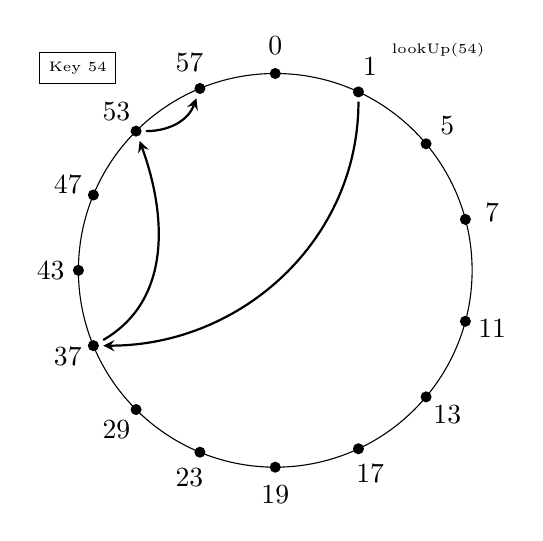
\begin{tikzpicture}
					\coordinate (center) at (1,2);
 					\def\radius{2.5cm}
  					% a circle
  					\draw (center) circle[radius=\radius];

  					% points on the circle
  					\fill[black] (center) ++(90:\radius) circle[radius=2pt] ++(90:1em) node {0};
  					\fill[black] (center) ++(65:\radius) circle[radius=2pt] node (One) {} ++(65:1em) node (text1) {1};
  					\fill[black] (center) ++(40:\radius) circle[radius=2pt] ++(40:1em) node {5};
  					\fill[black] (center) ++(15:\radius) circle[radius=2pt] ++(15:1em) node {7};
  					\fill[black] (center) ++(-15:\radius) circle[radius=2pt] ++(-15:1em) node {11};
  					\fill[black] (center) ++(-40:\radius) circle[radius=2pt] ++(-40:1em) node {13};
  					\fill[black] (center) ++(-65:\radius) circle[radius=2pt] ++(-65:1em) node {17};
  					\fill[black] (center) ++(-90:\radius) circle[radius=2pt] ++(-90:1em) node {19};
  					\fill[black] (center) ++(-112.5:\radius) circle[radius=2pt] ++(-112.5:1em) node {23};
  					\fill[black] (center) ++(-135:\radius) circle[radius=2pt] ++(-135:1em) node {29};
  					\fill[black] (center) ++(-157.5:\radius) circle[radius=2pt] node (Thirtyseven) {} ++(-157.5:1em) node {37};
  					\fill[black] (center) ++(-180:\radius) circle[radius=2pt] ++(-180:1em) node {43};
  					\fill[black] (center) ++(157.5:\radius) circle[radius=2pt] ++(157.5:1em) node {47};
  					\fill[black] (center) ++(135:\radius) circle[radius=2pt] node (Fiftythree) {} ++(135:1em) node (text53) {53};
  					\fill[black] (center) ++(112.5:\radius) circle[radius=2pt] node (Fiftyseven) {} ++(112.5:1em) node {57};
  					
  					%textboxes
  					\node[draw, above left, yshift=1em] at (text53) {\tiny Key 54};
  					\node[anchor=south west, xshift=1ex] at (text1) {\tiny lookUp(54)};
  					
  					%arrows
  					\draw[arrow] (One) edge[out=-90,in=0,->] (Thirtyseven);
  					\draw[arrow] (Thirtyseven) edge[out=30,in=-70,->] (Fiftythree);
  					\draw[arrow] (Fiftythree) edge[out=0,in=-110,->] (Fiftyseven);
				\end{tikzpicture}
			\end{adjustwidth}
		\end{adjustwidth}
	\end{adjustwidth}
	
	\section*{3.5 How does a specific P2P network deal with high churn rates?}
	\begin{adjustwidth}{2em}{2em}
	\end{adjustwidth}
\end{document}